\chapter{Generative-Adversarial-Networks}\label{chapter:gans}
In Machine-Learning existieren viele verschiedene Modelle, die vorhandene
Datensätze analysieren und anhand der Daten lernen, Strukturen in den
Datensätzen zu erkennen.  Besitzt man beispielsweise einen Datensatz
bestehend aus Fotoaufnahmen von Tieren, so kann ein Klassifizierer trainiert
werden, um einem Bild eine Tierklasse zuzuweisen. Aus diesem Grund fässt man
diese Modelle unter dem Begriff \textit{Bildklassifizierung} zusammen.

Wesentlich interessanter ist das Erkennen von vielen Objekten innerhalb eines
Bildes, anstatt das gesamte Bild nur einer einzigen Klasse zuzuweisen. In der
\textit{Objekterkennung} entwickelt man Modelle, welche mehr als nur eine
Klasse erkennen können. Sie liefern zusätzlich zu den erkannten Klassen ihre
Position und Größe innerhalb des Bildes. Diese Modelle treffen also keine
Aussage über das Gesamtbild, sondern treffen Aussagen über einzelne Objekte
innerhalb des Bildes.

Neben Modellen, die zu einem bestimmten Sachverhalt eine Aussage treffen
können, existieren auch Modelle, welche in der Lage sind, neue Sachverhalte zu
erzeugen. Diese fallen unter dem Begriff \textit{Generative Adversarial
Networks} (GANs) und bilden das Hauptthema dieses Abschnitts. Das interessante
an diesen generativen Modellen ist, dass sie nicht nur die Strukturen eines
Datensatzes lernen, sondern darüber hinaus neue Elemente der
Ausgangsdistribution erzeugen können. Trainiert man also ein generatives
Modell auf einen Datensatz, welcher Bilder von verschiedenen Tieren enthält,
können neue Bilder der gleichen Art erzeugt werden.

Aber nicht nur zum Erzeugen von Bildern kann diese Art von Modellen verwendet
werden. Auch bei Aufgaben, bei denen eine Voraussagung getroffen werden soll,
werden generative Modelle eingesetzt. Beispielsweise wurde in
\cite{barsoum2017hpgan} gezeigt, wie zu bereits getätigten menschlichen
Bewegungen unterschiedliche, darauf folgende Bewegungssequenzen aussehen
können. Hier hat man also versucht, eine Vorhersage zur Entwicklung von
menschlichen Bewegung zu tätigen.

Die Funktionsweise von GANs ist im Prinzip ziemlich simpel. Während beim
klassischen supervised-learning in der Regel nur ein Modell beim Training
involviert ist, verhält sich das bei generativen Modellen etwas anders. Zum
Einen wird ein Generator definiert, welcher, wie sein Name andeutet, Ausgaben
selbst erzeugt. Zum Anderen wird ein Diskriminator in das Training eingebaut,
welcher zwischen künstlich erzeugten und reellen Daten unterscheidet. Diese
beiden Modelle werden dann gleichermaßen trainiert. Während der Generator
versucht, Fälschungen immer genauer zu erzeugen, versucht der Diskriminator
immer besser zwischen Fälschung und Realität zu unterscheiden. Die
Ausgabe des Diskriminators ist dementsprechend entweder 0 für Fälschung und 1
für Realität. Mit anderen Worten, die beiden Komponenten spielen Spiel, in
welchem die eine Partei versucht, die andere zu täuschen
\cite{goodfellow2014generative}.
\[
\min_G \max_D V(G, D) = \mathbb{E}_{x \sim p_{data}(x)}\left[ \log D(x) \right] + \mathbb{E}_{z \sim p_z(z)}\left[ \log (1 - D(G(z))) \right]
\]

Der Eingabeparameter $z \in \mathbb{R}^n$ stellt einen $n$-dimensionalen Vektor
dar, welcher auch als latenter Vektor bezeichnet wird. Dementsprechend wird der
Vektorraum auch als latenter Raum bezeichnet. Ein solcher Vektor repräsentiert
verschiedenste Objekte mithilfe seiner $n$ Komponenten. In Bezug zu GANs wurde
festgestellt, dass ein GAN nicht nur lernt, ähnliche Daten zu einem bestehenden
Datensatz zu erzeugen, sondern auch den Zusammenhang zwischen latenten
Komponenten und einer Ausgabe zu verstehen. Das schöne daran ist, dass diese
latenten Vektoren mithilfe der Gesetze aus der linearen Algebra analysiert und
entsprechende Operationen mit ihnen ausgeführt werden können. Hierzu kann
folgendes, sehr einfaches Experiment durchgeführt werden. Man wählt zwei
latente Vektoren $a, b \leftarrow \mathbb{R}^n$, wobei die Komponenten dieser
Vektoren gleich sind, also $a_i = b_i, \; 0 \leq i < n$. Nun wählt man einen
zufälligen Komponentenindex $j \in \mathbb{N}$ mit $j \in \left[0, n\right[$
und wählt einen zufälligen Wert für die Komponenten beider Vektoren $a_j
\leftarrow \mathbb{R},\; b_j \leftarrow \mathbb{R}$, wobei $a_j \neq b_j$.
Betrachtet man nun die Ausgaben des Generators mit $a$ und $b$ als Eingabe,
dann unterscheiden sich diese um die Eigenschaft, die durch die Komponente an
der Stelle $j$ beeinflusst wird. Das gleiche Prinzip kann auch rückwärts
durchgeführt werden. Erzeugt der Generator zum Beispiel ein Bild, worauf ein
Gesicht mit Brille zu sehen ist und ein weiteres Bild mit Gesicht ohne
Brille, dann kann man die beiden Eingabevektoren voneinander subtrahieren und
damit die Komponenten herausfinden, die für die entsprechenden Eigenschaften
zuständig sind (in diesem Fall, ob das Gesicht eine Brille trägt oder nicht).

Im Verlauf des Trainings entwickelt sich damit ein Generator, welcher im
Idealfall so gute Fälschungen erzeugt, sodass sich diese nicht mehr von Daten
der Ausgangsdistribution unterscheiden lassen. Der Diskriminator kann hier
bestenfalls nur raten, kann also eine Genauigkeit von höchstens 50\%
erreichen. Ist dies nicht der Fall, d.h. der Diskriminator kann Fälschungen
mit einer höheren Wahrscheinlichkeit von realen Daten unterscheiden, so
entsteht ein Ungleichgewicht. Aus diesem Grund sollten die Lernparameter
sorgfältig ausgewählt und untersucht werden, damit ein stabil laufendes GAN
trainiert wird.

\section{Das Mode-Collapse-Problem}
Ein großes Problem beim Trainieren von generativen neuronalen Netzen ist, dass
sich der Generator sehr häufig auf bestimmte Merkmale der Ausgangsdistribution
des Datensatzes fixiert. Das Ergebnis sind signifikant erhöht wiederkehrende
Ergebnisse, die sich kaum bis gar nicht von anderen Ausgaben unterscheiden.
Man erwartet jedoch, dass das jeweilige GAN eine vielseitige Variation aus
allen Elementen des Datensatzes erzeugt. Mit anderen Worten, bei einer
zufälligen Eingabe in das Netz, soll immer eine unterschiedliche Ausgabe
erzeugt werden. Bei einem Mode-Collapse ist dies nicht der Fall. Es kann
beispielsweise passieren, dass wenn das Netz auf das Erzeugen von neuen
Gesichtern trainiert wird, dass dieses ausschließlich weibliche Gesichter
erzeugt, weil das Netz herausgefunden hat, dass es einfacher ist, weibliche
Gesichtszüge zu generieren, als männliche \cite{richardson2018gans}. Dies
lässt sich damit erklären, dass der Generator beim Trainingsvorgang mehr
Erfolg beim Generieren von weiblichen Gesichtern hatte und der Diskriminator
es schwerer hatte, Fälschung von Realität zu unterscheiden. Um das Problem zu
beseitigen wurden einige Erweiterungen an dem Standardmodell des GAN von
\cite{goodfellow2014generative} hinzugefügt.

\section{Deep-Convolution-GAN}
Das \textit{Deep Convolution GAN} (DCGAN) ist ein Versuch,
\textit{Convolutional Neural Networks} (CNNs) mit GANs zu verknüpfen. Nach
vielen Fehlschlägen in der Entwicklung von GANs mit CNNs ist die Version von
\cite{radford2016unsupervised} stabil und auf viele unterschiedliche
Datensätze anwendbar. Dafür wurden viele verschiedene Kombinationen von
Schichten untersucht und es wurde dabei eine Architektur ausgearbeitet, die
in ein stabiles Training über verschiedenste Datensätze resultierte.
Zusätzlich können mithilfe dieser Architektur höhere Auflösungen und tiefere
Netze erreicht werden.

Zusätzlich zur eigentlichen Architektur von DCGAN werden moderne Techniken
verwendet, um CNN-Architekturen zu vereinfachen.  Damit der Generator über
mehrere Schichten hinweg die räumliche Darstellung von Objekten lernen kann,
werden Convolutional-Layer verwendet. Anstatt, dass sogenannte
Max-Pooling-Layer zum Einsatz kommen, können nach
\cite{springenberg2015striving} einfach Convolutional-Layer mit erhöhtem
Stride verwendet werden, ohne dass die Genauigkeit sinkt. In Bezug zu DCGANs
von \cite{radford2016unsupervised} werden solche Schichten verwendet, um dem
Generator das Erlernen vom räumlichen Upsampling zu ermöglichen. Auch der
Diskriminator wird mit solchen CNN-Layer ausgestattet, um räumliches
Downsampling zu erlernen.

Neben dem Auslassen von Max-Pooling-Layer folgt DCGAN auch dem Trend,
Fully-Connected-Layer vor jedem Convolutional-Feature zu vermeiden. Dabei
wurde festgestellt, dass die Verknüpfung von Fully-Connected-Layer und der
Eingabe des Generators bzw. mit der Ausgabe des Diskriminators am besten
funktionieren. Die erste Schicht des Generators ist also ein
Fully-Connected-Layer (1-dimensional), jedoch wird die Ausgabe der Schicht in
einen 4-dimensionalen Tensor umgewandelt. Im Falle des Diskriminators wird die
Ausgabe des letzen Convolutional-Layers (4-dimensional) abgeflacht und in eine
1-dimensionale Schicht mit einer Sigmoid-Aktivierungsfuntion gefüttert
\cite{radford2016unsupervised}.

Um Mode-Collapse zu vermeiden, verwendet \cite{radford2016unsupervised}
Batch-Normalization-Layer. Dadurch wird das Training stabilisiert und Probleme
wie \textit{Internal-Covariate-Shifting} angegangen \cite{pmlr-v37-ioffe15}.
Vor allem wird dadurch aber auch verhindert, dass der Generator immer die
gleichen Ausgaben erzeugt. Das Anwenden der Batch-Normalisierung in allen
Schichten des Netzwerks führt jedoch zur Stichprobenoszillation und
Instabilität des Modells. Aus diesem Grund wird auf Batch-Normalization in der
Ausgabesschicht des Generators und in der Eingabeschicht des Diskriminators
verzichtet.

Als letzte Beobachtung stellt \cite{radford2016unsupervised} fest, dass das
Hinzufügen von ReLU-Ak\-ti\-vier\-ungs\-funk\-tio\-nen in allen Schichten des
Generators zu schnellerem Lernen und Abdeckung der Farbräume der
Trainingsdistribution führt. In der Ausgabeschicht wird jedoch anstatt von
ReLU-Aktivierung eine Tanh-Aktivierung verwendet. Innerhalb des Diskriminators
werden schließlich Leaky-ReLU-Aktivierungen angewandt.

\begin{figure}
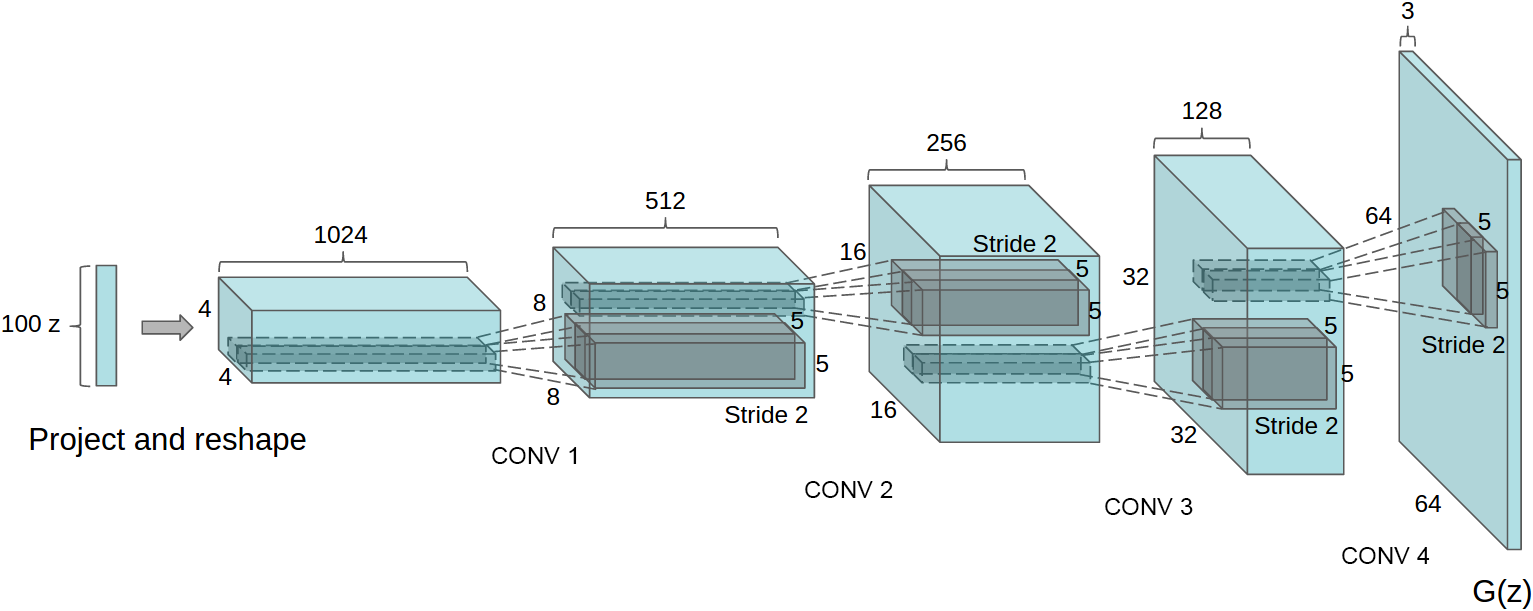
\includegraphics[width=\textwidth]{images/dcgan-architecture}
\caption{DCGAN-Architektur des Generators von
\cite{radford2016unsupervised}. Als Eingabe dient ein 100-dimensionaler
Vektor, dessen Elemente zufällig gewählt werden. Dieser wird dann in den
ersten Schichten umgeformt und durch vier Convolutional-Layer auf die Form
3$\times$64$\times$64 gebracht. Die Strides geben dabei den
Vergrößerungsfaktor pro Convolution-Schicht an, während die Anzahl der
Filter den Farbkanälen entsprechen.}
\end{figure}

\section{Wasserstein-GAN}
Anders als andere GAN-Varianten verwendet das Wasserstein-GAN (WGAN) die
Was\-ser\-stein-Distanz anstelle der JS- oder KL-Divergenz, um die Gewichte
von generativen neuronalen Netzen zu optimieren. Da sich die Berechnung aller
möglichen gemeinsamen Verteilungen $\gamma \sim \Pi(P_r, P_\theta)$ etwas schwierig
gestaltet, formt \cite{arjovsky2017wasserstein} die Definition unter
Berücksichtigung der Kontorovich-Rubinstein-Dualität um, sodass
\[
W(P_r, P_\theta) = \sup_{\|f\|_L \leq 1} \mathbb{E}_{x \sim P_r}\left[f(x)\right] - \mathbb{E}_{x \sim P_\theta}\left[f(x)\right]
\]

gilt, wobei das Supremum über alle 1-Lipschitz-Funktionen $f : X \to
\mathbb{R}$ ist. Zusätzlich wird ein kleiner Trick angewendet, um das Problem
weiter zu vereinfachen, indem K-Lipschitz-kontinuierliche Funktionen verwendet
werden.
\[
K \cdot W(P_r, P_\theta) = \sup_{\|f\|_L \leq K} \mathbb{E}_{x \sim P_r}\left[f(x)\right] - \mathbb{E}_{x \sim P_\theta}\left[f(x)\right]
\]

Nehmen wir nun an, dass die Abbildung $f \in \left\{f_w\right\}_{w \in W}$
parametrisiert durch $w$ existiert, wobei $W$ die Menge aller möglichen
Parameter darstellt, so können die Parameter $w$ und damit die Abbildung $f_w$
von einem neuronalen Netz erlernt werden, um so die Wasserstein-Distanz
effizient abzuschätzen. Hier bildet der Wasserstein-Abstand also gleichzeitig
die Loss-Funktion des Kritisierer mit
\[
W(P_r, P_\theta) = \max_{w \in W} \mathbb{E}_{x \sim P_r}\left[f_w(x)\right]
- \mathbb{E}_{z \sim P_r(z)}\left[f_w(g_\theta(z))\right].
\]

Trotzdem darf nicht vergessen werden, dass dies nur gültig ist, falls die
Funktion 1-Lipschitz-kontinuierlich ist. Um dies zu erzwingen, werden die
Werte der aktualisierten Gewichte des Kritisierer zwischen $\left[-c; c\right]$
gehalten. Dabei muss laut \cite{arjovsky2017wasserstein} $c$ relativ klein
sein.

\begin{algorithm}
\SetAlgoLined
\KwIn{Lernrate $\alpha$, Clipping-Parameter $c$, Batch-Größe
$m$, Anzahl von Kritisierer-Iterationen $n_{critic}$.}
\KwResult{Trainieren der Kritisierer-Parameter
$w$ und Generator-Parameter $\theta$.}
\caption{Wasserstein GAN nach \cite{arjovsky2017wasserstein}. Standardwerte
für die Eingabeparameter sind $\alpha = 5\cdot10^{-5}, c = 0.01, m = 64$
und $n_{critic} = 5$.}
\label{alg:wgan}
\BlankLine

\While{$\theta$ \textnormal{ist nicht konvergiert}}{
    \For{$t = 0, ..., n_{critic}$}{
    Erzeuge Batch $\left\{x_i \;\lvert\; 1 \leq i \leq m\right\} \sim
    \mathbb{P}_r$ aus realen Daten\;
    Erzeuge Batch $\left\{z_i \;\lvert\; 1 \leq i \leq m\right\} \sim
    \mathbb{P}_z$ aus latenten Vektoren\;
    \BlankLine
    $g_w \leftarrow
    \nabla_w \left[ \frac{1}{m}\sum_{i=1}^{m} f_w(x_i) -
    \frac{1}{m}\sum_{i=1}^{m} f_w(g_\theta(z_i)\right]$\;
    \BlankLine
    $w \leftarrow w + \alpha \cdot \mathrm{RMSProp}(w,
    g_w)$\;
    $w \leftarrow \mathrm{clip}(w, -c, c)$\;
    }
    \BlankLine
    Erzeuge Batch $\left\{z_i \;\lvert\; 1 \leq i \leq m\right\} \sim
    \mathbb{P}_z$ aus latenten Vektoren\;
    $g_\theta \leftarrow -\nabla_\theta \left[\frac{1}{m} \sum_{i=1}^{m}
    f_w(g_\theta(z_i))\right]$\;
    $\theta \leftarrow \theta - \alpha \cdot \mathrm{RMSProp}(\theta,
    g_\theta)$\;
}
\end{algorithm}

Zusätzlich ist bei Wasserstein-GANs von einem Kritisierer (Critic) anstatt
eines Diskriminators die Rede. Der Grund dafür ist, dass ein Diskriminator
zwischen \textit{fake} und \textit{real} unterscheidet, mehr nicht. Der
Kritisierer führt diese Unterteilung der Eingabeparameter nicht durch, sondern
bewertet bzw. kritisiert diese viel mehr. Mathematisch ausgedrückt sprechen
wir hierbei von einer linearen Ausgabe in $\mathbb{R}$ im Falle des
Kritisierers, während der Diskriminator eine binäre Ausgabe erzeugt.  Zu
Beginn von Algorithmus \ref{alg:wgan} werden die Parameter $w$ für den
Kritisierer und $\theta$ für den Generator initialisiert. Anschließend werden
$m$ Datenpunkte bzw. ein Batch aus dem reellen Datensatz (Verteilung
$\mathbb{P}_r$) gezogen. Dies muss nicht unbedingt zufällig sein. Auch werden
$m$ zufällige Vektoren erzeugt, die als Eingabe für den Generator dienen,
welcher wiederum Fake-Daten erzeugt. Dabei bilden die Ausgaben des Generators
eine eigene Verteilung $\mathbb{P}_\theta$.  Ziel des Generators ist es nun,
die Distanz zwischen den beiden Verteilungen $\mathbb{P}_r, \mathbb{P}_\theta$
zu minimieren, um möglichst realitätsnahe Ausgaben erzeugen zu können. Als
nächstes werden die Gradienten $g_w$ für Parameter $w$ mithilfe von
Gradient-Descent, dargestellt als $\nabla_w$, berechnet. Hierfür wird die
Wasserstein-Distanz als Loss-Funktion verwendet.  Der nächste Schritt besteht
daraus, die Parameter $w$ des Kritisierer-Netzwerks mithilfe des
RMSprop-Algorithmus zu aktualisieren und die aktualisierten Gewichte so gering
wie möglich zu halten, um die K-Lipschitz-Kontinuität zu gewährleisten. Dies
wird mithilfe der Funktion $\mathrm{clip}$ umgesetzt, welche die
Parameterwerte in einem bestimmten Intervall $\left[-c; c\right]$ festsetzt.
Die bis hier erläuterten Schritte werden $n_{critic}$-mal durchgeführt, sodass
das Kritisierer-Netzwerk immer öfter trainiert wird, als der Generator. Dieser
wird nun optimiert, indem wieder $m$ Vektoren zufällig erzeugt und als Eingabe
für das Generator-Netzwerk verwendet werden. Der Generator erzeugt damit $m$
zufällige Ausgaben, die wiederum als Eingaben in das Kritisierer-Netzwerk
gegeben werden. Aus den Ausgaben wird dann der Mittelwert gebildet und zum
Bestimmen der Gradienten von den Generator-Parametern $\theta$ verwendet.

Im direkten Vergleich zu dem originalen GAN \cite{goodfellow2014generative}
werden einige Änderungen in der Architektur vorgenommen. Während in dem
originalen Anstatz fast nach jeder Schicht eine Batch-Normalization
vorgenommen wird, können diese bei WGANs entfallen. Standard-GANs würden
hierbei kaum interpretierbare Resultate erzeugen, WGANs hingegen produzieren
trotzdem gute Ergebnisse, wie Experimente von \cite{arjovsky2017wasserstein}
zeigen (siehe Abbildung \ref{fig:wgan-gan-no-batchnorm}). Das Wasserstein-GAN
hat zusätzlich noch einige nützliche Eigenschaften. So wird unter anderem
durch Annäherung des Wasserstein-Abstandes zwischen Generator- und
Ausgangsdistribution das Problem des Mode-Collapse gelöst.  Durch den
Wasserstein-Abstand wird der Abstand zwischen den Verteilung wesentlich besser
minimiert (im Falle des Generator-Modells) als bei der KL- oder JS-Divergenz.
Die Ausgabe eines Kritisierers stellt damit eine Bewertung der Eingabe dar,
anstatt diese einer Klasse zuzuweisen und besitzt deshalb mehr Aussagekraft.

\begin{figure}
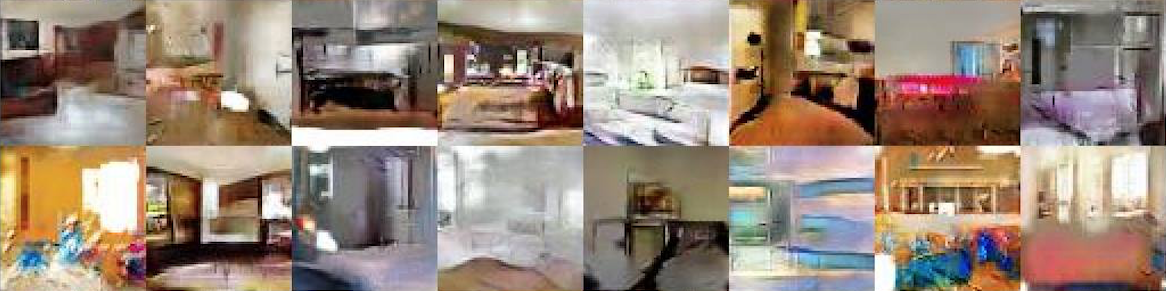
\includegraphics[width=0.5\textwidth]{images/image-022.png}
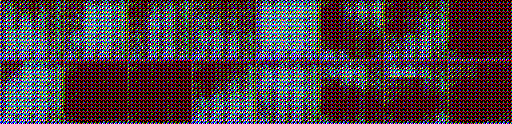
\includegraphics[width=0.5\textwidth]{images/image-024.png}
\caption{Vergleich von WGAN und Standard-GAN \cite{arjovsky2017wasserstein}.
    Links sind Ausgaben vom WGAN-Algorithmus zu sehen während rechts Ausgaben
    eines Standard-GANs dargestellt sind. In beiden Generator-Modellen wurden
    Batch-Normalization-Layer entfernt. Klar zu erkennen ist, dass WGAN immer
    noch interpretierbare Ergebnisse liefert während bei Standard-GANs Probleme
    erkennbar sind.}
\label{fig:wgan-gan-no-batchnorm}
\end{figure}

\section{Wasserstein-GAN mit Gradient-Penalty}
Ein großes Problem von Wasserstein-GANs ist das Clippen der Gewichte in ein
fest definiertes Intervall, um die 1-Lipschitzstetigkeit zu erfüllen. Das dies
keine elegante Lösung ist, liegt auf der Hand. In \cite{gulrajani2017improved}
wurde speziell dieses Problem genauer untersucht und es wurde festgestellt,
dass das Beschneiden der Gewichte den Kritisierer dazu verleitet, nur extrem
einfache Funktionen zu erlernen, wie der Vergleich in Abbildung
\ref{fig:problems-of-weight-clipping} zeigt. 

Um das Problem des Weight-Clippings anzugehen, stellt
\cite{gulrajani2017improved} eine alternative Lösung vor, die auf anderem Wege
die 1-Lipschitzstetigkeit in WGANs sicherstellen soll. Hierbei soll
Gradient-Penalty helfen und wird als
\[
(\|\nabla_{\hat{x}} D(\hat{x})\| - 1)^2
\]
berechnet, wobei $\hat{x} =  x \epsilon + \tilde{x}(1 - \epsilon)$ eine
zufällige Gewichtung zwischen realen ($x$) und generierten Daten ($\tilde{x}$)
darstellt. Das $\epsilon$ wird dabei zufällig aus $\left[0, 1\right]$ gewählt.
Daraus resultierend gestaltet sich die neue Loss-Funktion des Kritisierers wie
folgt.
\[
L = \mathbb{E}_{\tilde{x} \sim \mathbb{P}_g}\left[D(\tilde{x})\right] -
    \mathbb{E}_{x \sim \mathbb{P}_r}\left[D(x)\right] +
    \lambda \cdot \mathbb{E}_{\hat{x} \sim \mathbb{P}_{\hat{x}}}\left[(\|\nabla_{\hat{x}} D(\hat{x})\| - 1)^2\right]
\]
Der Kritisierer ist durch diese Änderung nun wesentlich besser dazu in der
Lage, komplexere Verteilungen zu erlernen.

\begin{algorithm}
\caption{WGAN mit Gradient-Penalty \cite{gulrajani2017improved}.}
\KwIn{Gradient-Penalty-Koeffizient $\lambda$, Anzahl von Kritisierer-Iterationen
$n_{critic}$, Batch-Größe $m$, Adam-Hyperparameter $\alpha, \beta_1,
\beta_2$.}
\KwResult{Trainieren der Kritisierer-Parameter $w$ und Generator-Parameter
$\theta$.}
\BlankLine
\While{$\theta$ \textnormal{ist nicht konvergiert}}{
    \For{$t = 1, ..., n_{critic}$}{
    \For{$i = 1, ..., m$}{
        Wähle reale Probe $x \sim \mathbb{P}_r$, latenten Vektor $\vec{z} \sim
        \mathbb{P}_z$, zufällige Zahl $\epsilon \in \left[0, 1\right]$\;
        $\tilde{x} \leftarrow G_\theta(\vec{z})$\;
        $\hat{x} \leftarrow x\epsilon + \tilde{x}(1 - \epsilon)$\;
        $L_i = D_w(\tilde{x}) - D_w(x) + \lambda(\|\nabla_{\hat{x}}
        D_w(\hat{x})\| - 1)^2$\;
    }
    \BlankLine
    $w \leftarrow \mathrm{Adam}(\nabla_w \frac{1}{m} \sum_{i=1}^m L_i, w,
    \alpha, \beta_1, \beta_2)$\;
    }
    \BlankLine
    Wähle einen Batch aus latenten Vektoren $\{\vec{z}_i\}_{i=1}^m \sim
    \mathbb{P}_z$\;
    $\theta \leftarrow \mathrm{Adam}(\nabla_{\theta} \frac{1}{m} \sum_{i=1}^m
    - D_w(G_\theta(\vec{z}_i)), \theta, \alpha, \beta_1, \beta_2)$\;
}
\end{algorithm}

\begin{figure}
\centering
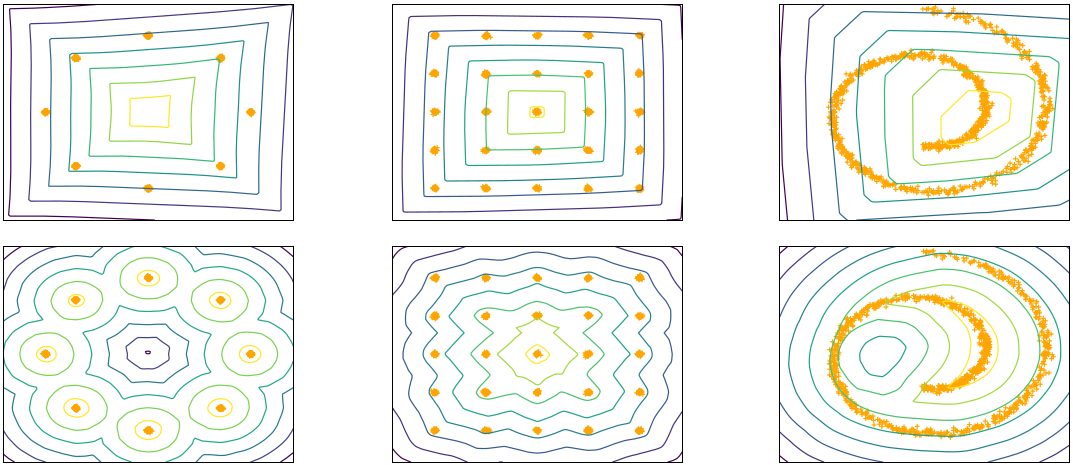
\includegraphics[width=\textwidth]{images/problems_of_weight_clipping}
\caption{Vergleich zwischen Weight-Clipping (oben) und Gradient-Penalty
(unten). Man erkennt deutlich, dass die Separierung der Ausgangsverteilung,
dargestellt durch orangene Punkte, durch Weight-Clipping in sehr
vereinfachte Funktionen resultiert. Gradient-Penalty lässt hingegen
komplexere Strukturen von Verteilungen zu \cite{gulrajani2017improved}.}
\label{fig:problems-of-weight-clipping}
\end{figure}

\section{Conditional-Wasserstein-GAN mit Gradient-Penalty}
Generative Modelle wie das WGAN oder DCGAN erzeugen bei einem zufälligen
Eingabevektor immer ein zufälliges, interpoliertes Element aus der
Trainingsdistribution. Besitzt der Trainingsdatensatz verschiedene Klassen, so
werden diese Modelle auch zwischen den Klassen interpolierte Ergebnisse
erzeugen. Aber was ist, wenn wir ein zufälliges Element einer bestimmten Klasse
erzeugen wollen? Nehmen wir als Beispiel einen Datensatz bestehend aus Bildern
von Hunden und Katzen. Die bisher vorgestellten DCGANs und WGANs würden auf
diesen Datensatz trainiert werden und würden bei einem zufälligen Eingabevektor
Hunde oder Katzenbilder bzw. eine Mischung aus beidem erzeugen. Möchte man nun
jedoch den Generator der GANs dazu bringen, nur zufällige Hundebilder zu
erzeugen, so muss aufwändig die dafür zuständige Komponente des Eingabevektors
extrahiert werden, die bestimmt, ob der Generator ein Hunde- oder ein Katzenbild
erzeugen soll. Eine einfachere Möglichkeit besteht darin, dem Generator
zusätzlich zum latenten Vektor die Klasse der zu erzeugenden Ausgabe zu
übergeben. Diese Idee wurde erstmals mit
Conditional-Generative-Adversarial-Networks (cGANs) \cite{mirza2014conditional}
umgesetzt und stellt eine Erweiterung zu den bisher besprochenen GANs dar.

Wie bereits erwähnt, wird bei cGANs zusätzlich zum latenten Vektor $x$ das Label
bzw. die Klasse $y$ als Eingabe verwendet. Wie dies technisch umgesetzt wird,
soll das Schema in Abbildung \ref{fig:cgan} verdeutlichen.

\[
\min_G \max_D V(G, D) = \mathbb{E}_{x \sim p_{data}(x)}\left[ \log D(x \lvert y) \right] + \mathbb{E}_{z \sim p_z(z)}\left[ \log (1 - D(G(z \lvert y))) \right]
\]

\begin{figure}
    \centering
    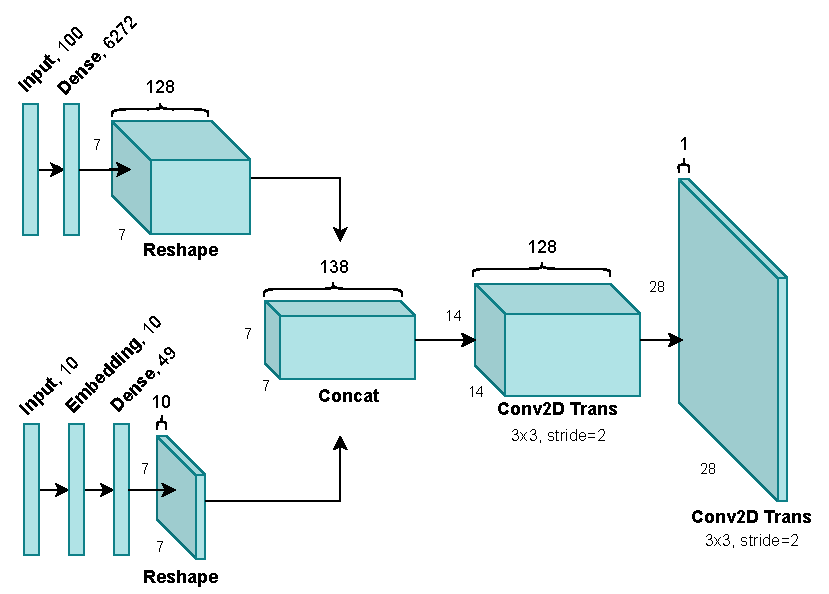
\includegraphics[width=0.7\textwidth]{images/cgan.pdf}
    \caption{Schematische Darstellung eines einfachen Conditional-GANs für den MNIST-Datensatz. Die Eingabe sind ein latenter Vektor mit 100 Komponenten und ein Labelvektor mit 10 Komponenten (entsprechend der Anzahl der Klassen).}
    \label{fig:cgan}
\end{figure}